\documentclass[12pt, letterpaper, titlepage]{article}

\usepackage{amsmath}
\usepackage{booktabs}
\usepackage{amsthm}
\usepackage{graphicx}
\usepackage[margin=1in]{geometry}
\usepackage{hyperref}
\hypersetup{colorlinks = true, linkcolor = blue, citecolor=blue, urlcolor = blue}
\usepackage{natbib}
\usepackage{enumitem}
\usepackage{setspace}

\usepackage[pagewise]{lineno}
%\linenumbers*[1]
% %% patches to make lineno work better with amsmath
\newcommand*\patchAmsMathEnvironmentForLineno[1]{%
 \expandafter\let\csname old#1\expandafter\endcsname\csname #1\endcsname
 \expandafter\let\csname oldend#1\expandafter\endcsname\csname end#1\endcsname
 \renewenvironment{#1}%
 {\linenomath\csname old#1\endcsname}%
 {\csname oldend#1\endcsname\endlinenomath}}%
\newcommand*\patchBothAmsMathEnvironmentsForLineno[1]{%
 \patchAmsMathEnvironmentForLineno{#1}%
 \patchAmsMathEnvironmentForLineno{#1*}}%

\AtBeginDocument{%
 \patchBothAmsMathEnvironmentsForLineno{equation}%
 \patchBothAmsMathEnvironmentsForLineno{align}%
 \patchBothAmsMathEnvironmentsForLineno{flalign}%
 \patchBothAmsMathEnvironmentsForLineno{alignat}%
 \patchBothAmsMathEnvironmentsForLineno{gather}%
 \patchBothAmsMathEnvironmentsForLineno{multline}%
}

% control floats
\renewcommand\floatpagefraction{.9}
\renewcommand\topfraction{.9}
\renewcommand\bottomfraction{.9}
\renewcommand\textfraction{.1}
\setcounter{totalnumber}{50}
\setcounter{topnumber}{50}
\setcounter{bottomnumber}{50}

\newcommand{\jy}[1]{\textcolor{blue}{JY: #1}}
\newcommand{\eds}[1]{\textcolor{red}{EDS: (#1)}}


\title{Time Series Length at Which Block Bootstrapping is Effective for Estimation of Variance}

\author{Mathew Chandy\\
%   \href{mailto:mathew.chandy@uconn.edu}
% {\nolinkurl{mathew.chandy@uconn.edu}}\\
  Jun Yan\\[1ex]
  Department of Statistics, University of Connecticut\\
}
\date{}

\begin{document} 
\maketitle

\doublespace

\begin{abstract}
Block bootstrapping is a method that can be used for estimating a parameter of a time
series. It involves splitting a series into blocks (in order to account for the time
factor) and re-sampling the blocks to create many new bootstrapped time series.
This method becomes more effective as the length of the time series increases. 
The question for this study is how does one determine at what length the block
bootstrap method stops being effective to estimate a parameter of a time
series.

\bigskip
\noindent\sc{Keywords}:
block bootstrap;
\end{abstract}

\section{Introduction}
\label{sec:intro}

Block bootstrapping is a widely used method in Statistics. The concept for block 
bootstrapping was developed independently by \citet{hall1985resampling}, \citet{carlstein1986use}, and 
\citet{kunsch1989jackknife}. \citet{radovanov2014comparison} It has been applied to a variety of 
different fields such 
as econometrics \citep{mackinnon2006bootstrap} and meteorology \citep{varga2017generalised}. It can be used for 
situations in which there is temporal dependence, and the goal is the estimation or testing a hypothesis about a parameter. Assuming that the sample is infinitely 
large, the method will work perfectly. However, for a finite sample size, the method will 
not work as well as expected. \citet{hesterberg2015teachers} notes that while intervals based on the percentiles from nonparametric bootstrapping are more accurate than t-intervals for larger sample sizes, they are less accurate for smaller sample sizes. In the context of planning an applied 
statistical procedure, for which a large sample size is not always practical, it may be helpful to know at which sample size the method stops working at an acceptable level. 
The goal of this study is to find a threshold or range of sample sizes at whichblock bootstrap 
is no longer an effective method for estimating variance.

\citet{nevitt2001performance} find that a sample size of 200-1000 is usually sufficient for estimation using the bootstrap method (simple resampling with no blocks involved). However, block bootstrapping is a different situation altogether because the sample is split into blocks.

\citet{goncalves2005bootstrap} found that standard error estimates from block bootstrapping small 
samples 
may be significantly more accurate than inference from closed-form asymptotic estimates. That study focused on the estimation of a parameter within the context of linear regression. Still, the block bootstrap percentile confidence intervals under covered even for n = 1024. This study aims to find how small the sample size can be for time series (which has a dependence factor which can be compared to that of a linear regression) in order for the coverage rate to be close to the confidence level.

For this study, many block bootstrap simulations were conducted with RStudio. At the base
level, we are block-bootstrapping an auto-regressive process with true mean 0.
Bootstrapping is the term for creating new samples of the same size by re-sampling from
the original sample with replacement. The means of many bootstrapped samples are used to create a
distribution of sampling means to estimate mean and variance. This works well for samples
that are do not have a dependence factor. However, for a time series such as an auto-regressive process,
a different procedure is required to account for the time dependence. In such a case,
the series is split into blocks that can overlap (moving block bootstrap) or not(non-moving block bootstrap). These blocks are then re-sampled to create a new
bootstrapped time series sample. 

In our experiment, we find the means of a 1000 block-bootstrapped time series, 
and create a 95 \% confidence interval of the means. We replicate this 1000 times, 
and record the proportion of confidence intervals that recover the true mean 
(coverage rate). We are effectively observing how successful the bootstrapping process
is at estimating the mean and variance. The key variable being observed was n, 
the length of the time series, or the size of the sample. It is known that as n
increases, block bootstrapping will become a less accurate method for estimation
(the coverage rates will decrease). The question is at what range of n values does this
start to become a problem. 

In this experiment, there are certain factors that are expected to affect the coverage
rates. As the Auto-Regressive (AR) coefficient (the time dependence) of the time series 
increases,
we expect the coverage rates of the confidence intervals to decrease.
The coverage rates are also affected by the size of the blocks - more specifically,
how the size of the blocks (l) relates to the size of the time series (n) - 
and whether or not they overlap. It is known that as the size of the time series 
increases, the optimal block length should increase, and the ratio of the block length to 
the time series length should decrease. l = n$^{1/3}$ is typically considered the optimal 
block length according to asymptotic theory. \citep{buhlmann1999block} The effect of the block function on the performance block bootstrap method was observed in this study. Simulations were conducted using block functions of l = 10 and l = n$^{1/3}$. 

In order to solve the question of what n is necessary for effective block bootstrapping,
while still accounting for all these factors, the simulations were repeated for
various combinations of AR coefficients, block length functions, and non-moving vs moving method. For each of these combinations, coverage rates were recorded for a wide range of sample sizes.

\section{Review of Block Bootstrap}
\label{sec:blkbootreview}

Block bootstrapping is a method that can be applied to a time series (or any sample of data for that matter) to estimate a parameter and its variance. Suppose that a sample of size n of a time series is given. In regular bootstrap procedure, the new sample of the same size as the original would just be created by resampling observations with replacement. In the case of a time series, in order to account for the temporal dependence, the time series can be split into blocks, typically of the same size. The block should be of size l large enough to include time dependence, yet small enough to include some variance. As n increases, an ideal l should also increase, but the ratio of l to n should decrease. To achieve this, l is often assigned a value as a function of n. A common function that is considered the best by much previous literature is l = n$^{1/3}$. However not all n sizes are perfect squares, and l must be a whole number, so the ceiling of this function must be used. A bootstrapped sample is created by taking a sample of n / l blocks with replacement to create a new series of size n. The designer of the study can choose whether the blocks overlap or not. If the blocks can never overlap, it is called a non-moving block bootstrap. In this case, the original sample is split evenly into n / l blocks, and the same number of blocks is sampled without replacement to create a bootstrapped sample. If the blocks do overlap, it is called a moving block bootstrap. n / l samples are taken randomly from the original sample, but they do not have to be from a set of evenly spaced blocks. An estimator of the parameter is computed from the bootstrapped sample. This procedure can be repeated many times (typically 1000) to create a sampling distribution of the estimator. Using this distribution of estimators, a 1 - $\alpha$/2 \% confidence interval for the parameter can be created using the $\alpha$/2 and 1 - $\alpha$/2 percentiles.

\section{Simulation Study Design}
\label{sec:simdesign}

The central objective of the study was to assess at which sample size the block bootstrap method no longer estimates the variance well for an autoregressive process. The method will work better as the sample size goes to infinity, but the goal is to see what is the smallest sample size that is acceptable. To achieve this, simulations must first be conducted with a larger sample size in order to compare to results with a smaller sample size. In the previous section, the procedure for creating a confidence interval using the block bootstrap method is described. This process is applied to a simulation of an autoregressive integrated moving average (ARIMA) with standard deviation = 0.1 to create a confidence interval of the mean of the process. R has a built in ARIMA simulation which allows you to set the AR coefficient and the standard deviation of the error term. Using the equation below, the sigma of the error term can be decided so that the standard deviation of Y is constant (0.1, Variance = 0.01). 

\[ \sigma_{x}^{2}=\sigma_{\eta}^{2}/\left( 1-\phi^2 \right)\]
\[\sigma_{\eta}=\sqrt{\sigma_{x}^{2}*\left( 1-\phi^2 \right)}\]

For a certain AR coefficient, a block bootstrap 95\% confidence interval is replicated 4000 times at a starting sample size at which block bootstrap is expected to be very effective (a relatively large sample). For each individual confidence interval, it can be recorded whether or not the interval includes the true mean (0). The coverage rate, or the proportion of intervals that include the mean, can then be recorded. If the parameter and its variance are being properly estimated by the block bootstrap, the coverage rate should reflect this by being close to the confidence level of 95\%. If this is not the case, the method is not working as well as it should. The width of the confidence interval for each replication is dependent on the variance of the means of the bootstrapped samples. If the interval is not wide enough to capture the mean at the expected rate of 95\%, it indicates that the variance of the parameter (which will be estimated from the variance of the means of the bootstrapped samples) will be underestimated. Since the coverage rate is a proportion based on many replication of independent Bernoulli outcomes, a 95\% confidence interval of the coverage rate at that sample size can also be created. Once the simulation is done for the starting n, the sample size can gradually be lowered until the coverage rates and their respective confidence intervals indicate that the method no longer functions well.

\section{Methods}
\label{sec:methods}

Before each set of 4000 replications of confidence intervals from block bootstrapped sample mean distributions, the random seed was set to 5 so that the randomized results can be 
reproduced. 

A simulation of an autoregressive integrated moving average (ARIMA) process was run 
repeatedly with varying parameters. 
The mean and standard deviation of the time series was held constant at 0 and 0.1, respectively, whereas 
the sample length and AR Coefficient
 were varied. The AR Coefficients that were observed with were 0.2, 0.4, and 0.6. Normally distributed samples, in other words, samples with AR Coefficients of 0, were also experimented with as a control group to compare against. The sample lengths 
 that were used depended on the AR
 Coefficient, but the lowest sample length observed was always n = 20.
 
 The block bootstrap method has different settings that were varied in this study: 
 non-moving vs moving, and the function for block length - the three functions used were l = 10 and l = f(n) = $\lceil n^{1/3} \rceil$. That means six variations of the block bootstrap method. 

For each simulated ARIMA process, the block bootstrap method with each of these six variations was applied to the sample. 4000 replications were conducted, meaning that 4000 samples of the same size from a process with the same parameters were simulated. For each sample, a 95\% confidence interval was created, and for each block bootstrap variation, the proportion of all 4000 intervals (created using that variation) that recovered the true mean (0) was recorded as the coverage
 rate for that specific variation. 95\% confidence intervals for these proportions were also computed.
 
For each AR coefficient, a starting sample size was decided based on expectations of how the bootstrap method would perform. Then, the sample size was gradually lowered by increments of 20 to see when
the block bootstrap would begin to consistently return low coverage rates. 

For both AR = 0 and AR = 0.2, results for sample sizes ranging from 400 to 20 were observed. For AR = 0.4, results for sample sizes ranging from 600 to 20 were observed. For AR = 0.6, results for sample sizes ranging from 900 to 20 were observed.

 

\section{Results}
\label{sec:results}

As the AR Coefficient increases, it was found unsurprisingly that a larger sample size was 
required for effective block bootstrap estimation. The tables below for each corresponding block length function and AR Coefficient display information about the length of the sample of the ARIMA process, the block length used in bootstrap, the method (non-moving or moving), and the proportion of 95\% confidence intervals produced by each of 4000 block bootstrap replications that recover the mean, as well as an interval in which we can be 95\% confident that the true coverage rate given an infinite number of replications is contained. 
As shown in the plots, as n decreases, the coverage rate decreases. As AR increases, not only is a larger sample size required for effective bootstrap estimation, but the level of noise also increases. The best block length function, as shown in previous literature \citep{buhlmann1999block}, is l = n$^{1/3}$, as it yields the most consistently high coverage rates even for samples as small as n = 20. l = 10 seems to perform almost as well as l = n$^{1/3}$ for higher sample sizes, but the coverage rates for l = 10 drop down much more for small sample sizes. For the larger sample sizes, there does not appear to be a significant difference in results for moving method vs non-moving method. However, block bootstrap with moving method appears to perform better for smaller sample sizes than block bootstrap with non-moving method.

\begin{figure}[tbp]
\caption{The figure below demonstrates how block bootstrap performs at estimating the mean of a normal population. As shown in the plots, even for a sample with no time dependency, a very large sample size is needed to even approach a coverage rate of 95\%.  While for large sample sizes (approximately greater than 300), the performance for l = 10 is comparable to the performance for l = n$^{1/3}$, the performance with l = 10 is much worse than that for l = n$^{1/3}$ when using very small sample sizes (approximately less than 100). The moving method seems to have a similar performance to the non-moving method, although it appears to perform slightly better for very low sample sizes regardless of the block length function.}
  \centering
  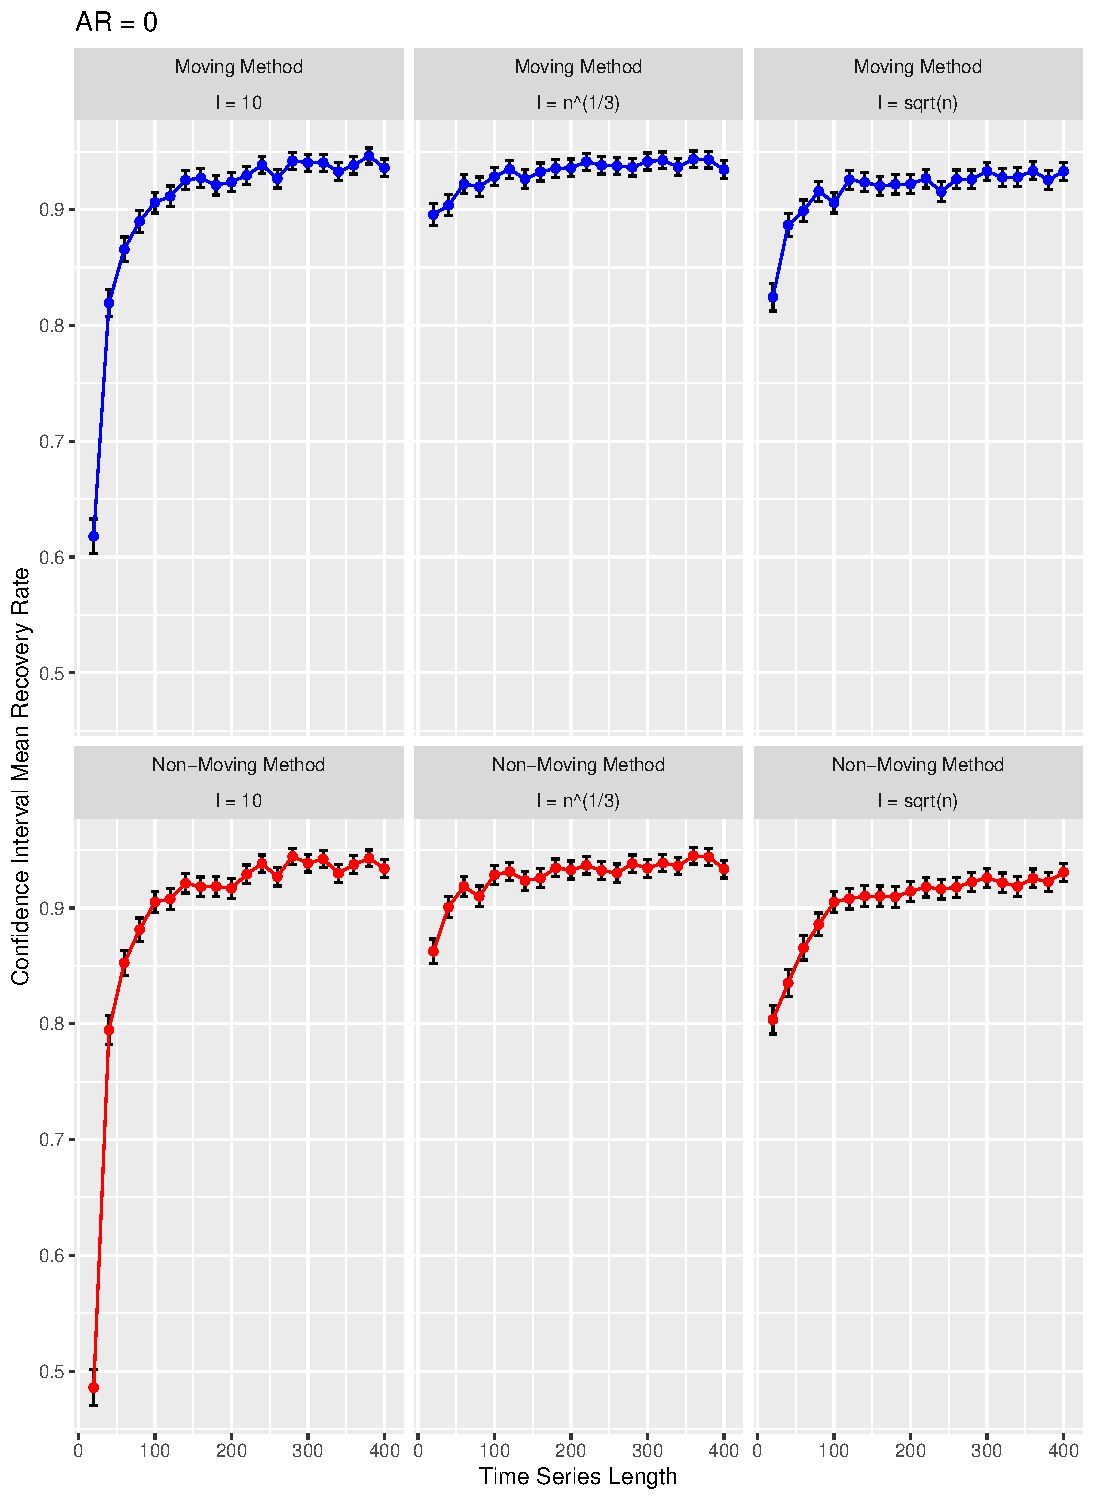
\includegraphics[width=\textwidth]{norm}
  \caption{}
  \label{fig:norm}
\end{figure}

\begin{figure}[tbp]
\caption{The figure below demonstrates how block bootstrap performs at estimating the mean of a AR = 0.2 process. As shown in the plots, even for a sample with relatively low dependency, a very large sample size is needed to even approach a coverage rate of 95\%.  While for large sample sizes (approximately greater than 200), the performance for l = 10 is comparable to the performance for l = n$^{1/3}$, the performance with l = 10 is much worse than that for l = n$^{1/3}$ when using small sample sizes (approximately less than 100). Again, the moving method seems to have a similar performance overall to the non-moving method, but the coverage rates drop off slightly more for non-moving method when using smaller sample sizes.}
  \centering
  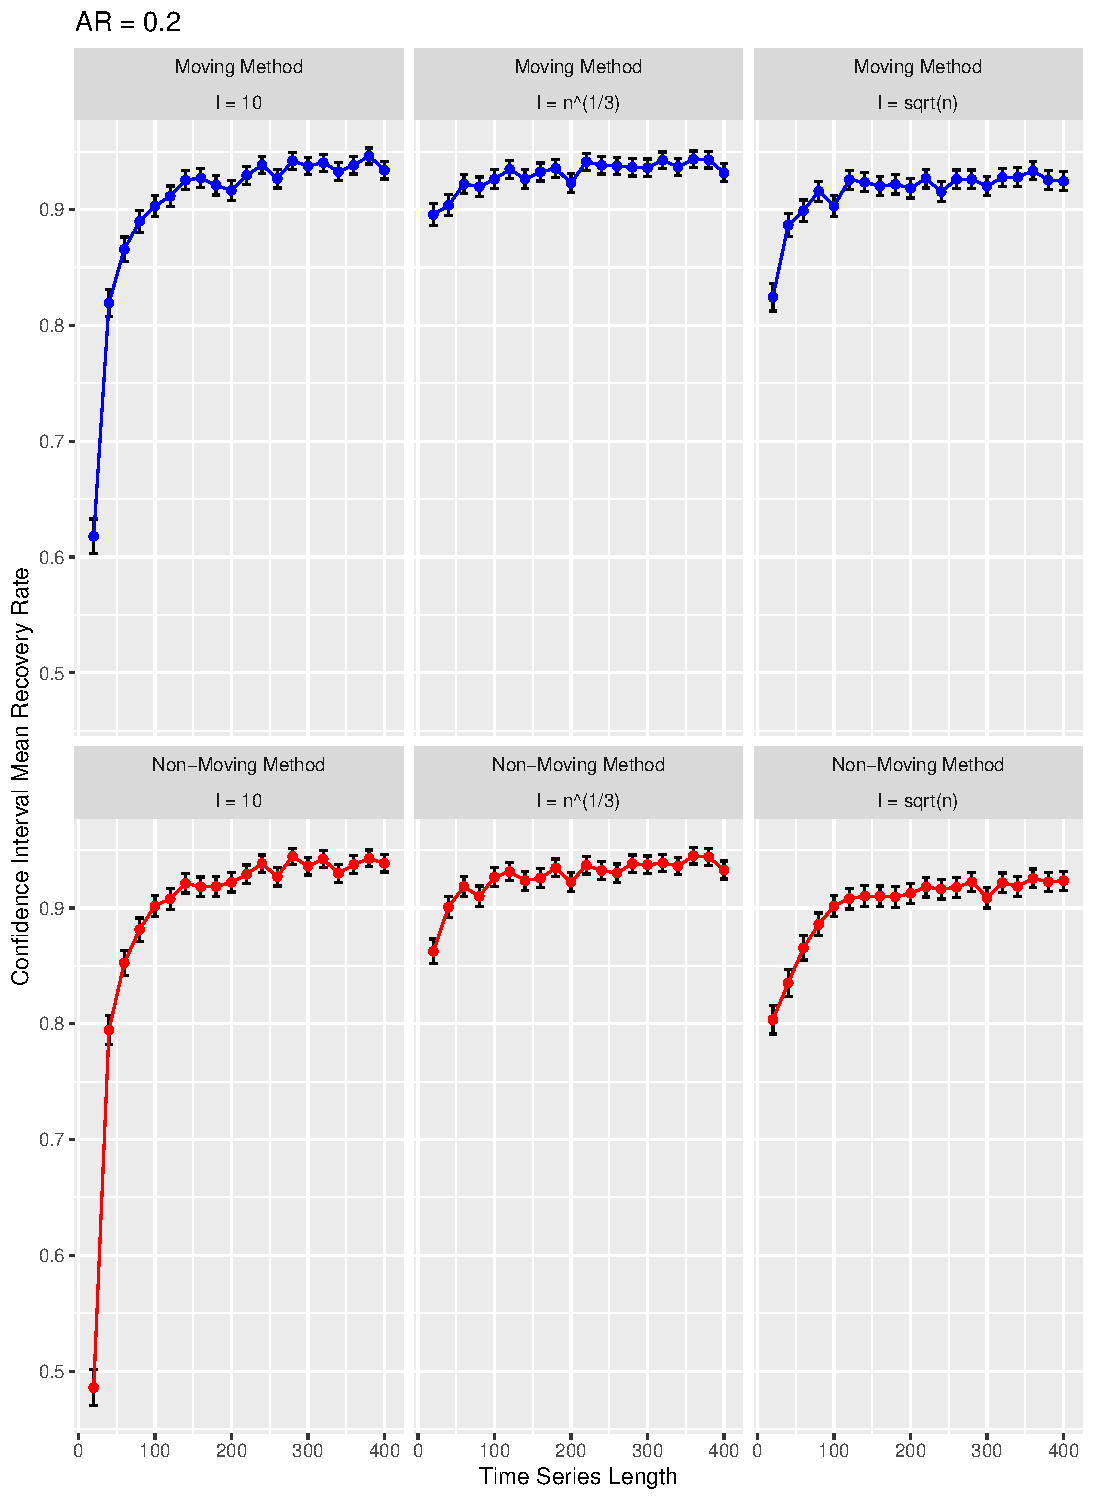
\includegraphics[width=\textwidth]{ar_0.2}
  \caption{}
  \label{fig:ar_0.2}
\end{figure}

\begin{figure}[tbp]
\caption{The figure below demonstrates how block bootstrap performs at estimating the mean of a AR = 0.4 process. As shown in the plots, even for a sample of size 600, the block bootstrap method fails to adequately capture the mean at a rate of \%.  While for large sample sizes, the performance for l = 10 is comparable to the performance for l = n$^{1/3}$, the performance with l = 10 is much worse than that for l = n$^{1/3}$ when using small sample sizes. Again, the moving method seems to have a similar performance overall to the non-moving method, but the coverage rates drop off slightly more for non-moving method when using smaller sample sizes.}
  \centering
  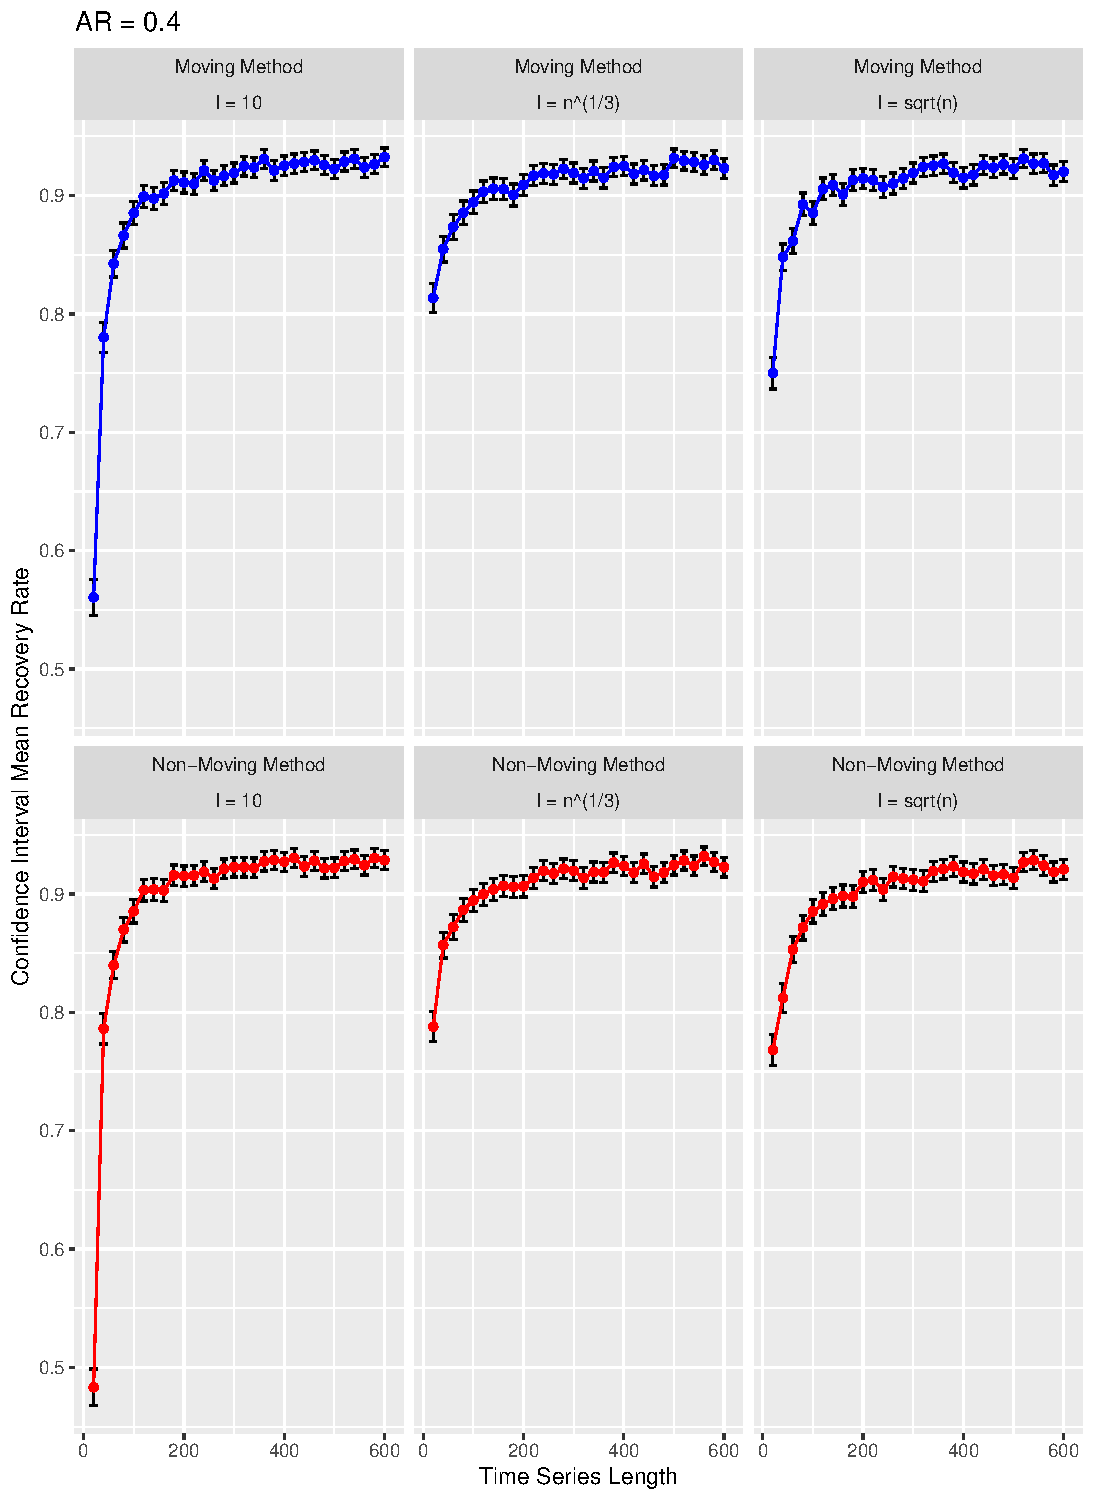
\includegraphics[width=\textwidth]{ar_0.4}
  \caption{}
  \label{fig:ar_0.4}
\end{figure}

\begin{figure}[tbp]
\caption{The figure below demonstrates how block bootstrap performs at estimating the mean of a AR = 0.6 process. As shown in the plots, even for a sample of size 900, the block bootstrap method fails to adequately capture the mean at a rate of 95\%.  While for large sample sizes, the performance for l = 10 is comparable to the performance for l = n$^{1/3}$, the performance with l = 10 is much worse than that for l = n$^{1/3}$ when using small sample sizes. Again, the moving method seems to have a similar performance overall to the non-moving method, but the coverage rates drop off slightly more for non-moving method when using smaller sample sizes, although the difference is less noticeable than for samples with lesser time dependence.}
  \centering
  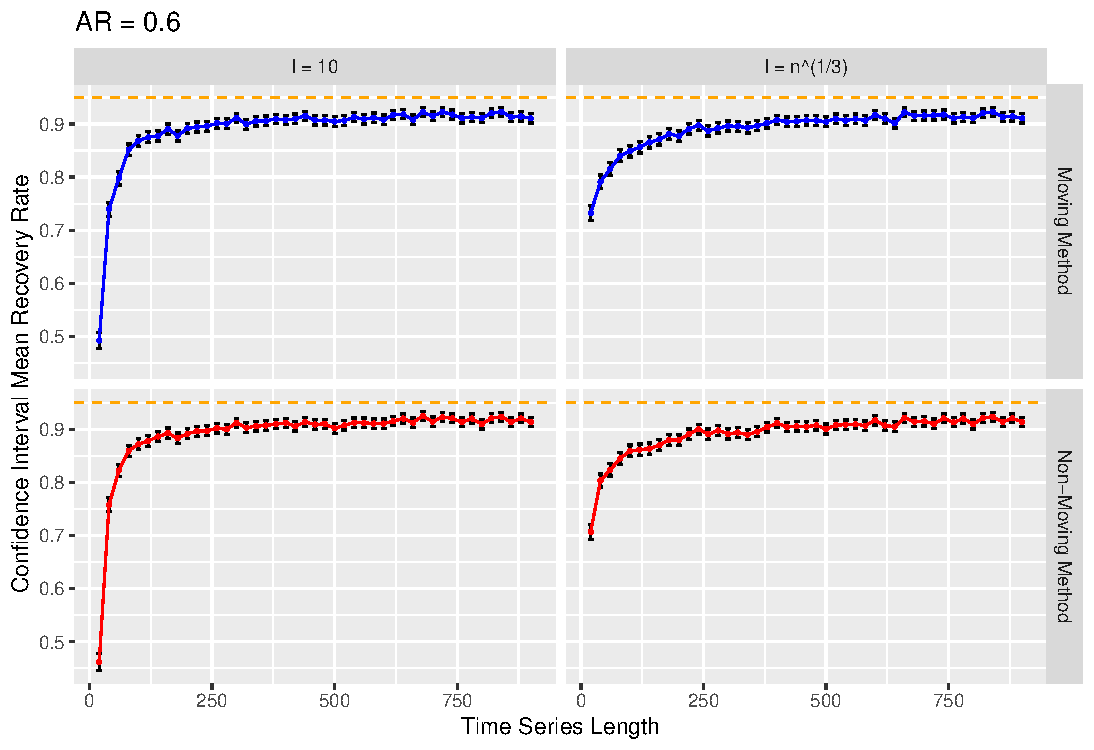
\includegraphics[width=\textwidth]{ar_0.6}
  \caption{}
  \label{fig:ar_0.6}
\end{figure}

\section{Discussion}
\label{sec:discuss}

This study finds that as the AR coefficient increases, the sample size necessary for effective block bootstrap estimation must be larger. When implementing the block bootstrap method using a block length function of l = n$^{1/3}$ results in the highest coverage rates overall (indicating a more accurate estimation of a parameter and its variance), but using l = 10 results in similar performance for large sample sizes. It is important to note that a different constant block length will perform differently for different ranges of sample sizes. While the moving-method and non-moving method yield similar coverage rates, the non-moving method performs slightly worse when using very small sample sizes.



\bibliographystyle{chicago}
\bibliography{citations}[tp]


\end{document}